\noindent\textbf{Resultado.} \[u(x,t)=\frac{\sin(ct)}c\cos x.\]
Para ct=0,\ensuremath{\pi}/2,\ensuremath{\pi},3\ensuremath{\pi}/2, los perfiles son respectivamente0,cosx/c,0,\ensuremath{-}cosx/c.
El período temporal fundamental es2\ensuremath{\pi}/c.

\noindent\textit{Desarrollo.} La fórmula de d’Alembert con posición inicial cero da
\[u(x,t)=\frac1{2c}\int_{x-ct}^{x+ct}\cos s\,ds
=\frac{\sin(x+ct)-\sin(x-ct)}{2c}=\frac{\sin(ct)}c\cos x.\]
La identidad de suma de senos muestra que el resultado es una onda estacionaria,
combinación de dos ondas viajeras opuestas. Directamente,
\(u_{tt}=-c\sin(ct)\cos x=c^2u_{xx}\), \(u(x,0)=0\), \(u_t(x,0)=\cos x\).
La solución es suave y global, y las fórmulas de propagación determinan de manera única
el PVI con estos datos. Los perfiles indicados fijan amplitud y signo en un ciclo.
Cuando \(c\to0^+\), \(\sin(ct)/c\to t\), que coincide con \(u_{tt}=0\) y los mismos datos iniciales.

La figura representa la magnitud escalada \(cu\) en cuatro instantes de un ciclo.
\begin{center}
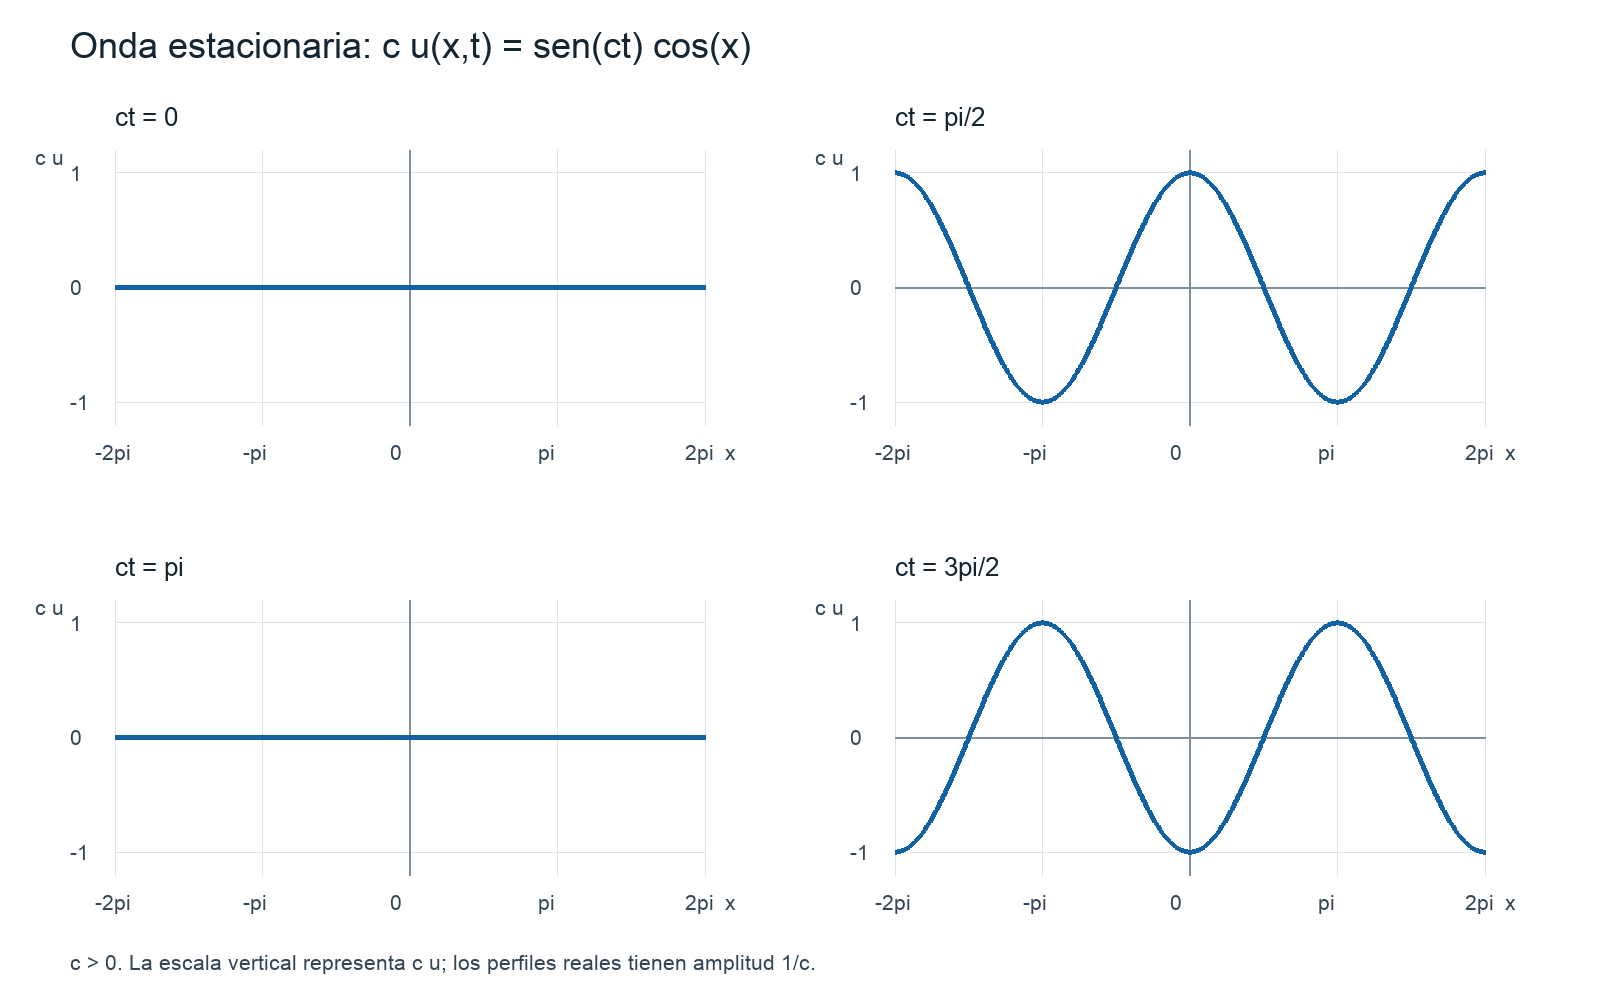
\includegraphics[width=.95\linewidth]{assets/M2-E0107-wave-profiles.png}
\end{center}
